\chapter{Displays}
\chaplabel{displays}

\section{Introduction}
Adding a display to a device allows much more information to be shared from the device to the user than 
just using LEDs or buzzers. There are several types of displays that are commonly used in the embedded systems 
world. 

\subsection{LCD}
The most common is a Liquid Crystal Display (LCD). Most of the computer monitors and computers are LCD. This 
technology gives good contrast, fast response (which gamers like), and minimal burn in. Old CRT displays had 
to have screensavers so that whatever was usually showing on the display wouldn't be there permanently. 
Thankfully modern displays don't typically have this problem. LCDs do require a backlight. This determines
how bright the colors are. The pixels in the display just modulate how much of the backlight is showing.

At times you will find TFT displays. This stands for thin-film-transistor liquid-crystal display. They are 
a better version of LCD.

\subsection{eInk}
eInk displays are also available for embedded systems. Kindles are probably the most popular commercial 
product using eInk type displays. These displays are of particular interest because they keep their 
display even when the power is turned off. This allows for very low power operations. The downsides are 
that they work off of reflected light so require special backlighting to be viewed at night and that 
they are very slow. A small display may take a second to refresh and some recommend not to update
them more than once every few minutes if possible.

\subsection{OLED}
The display in this class is based on Organic Light Emitting Diodes (OLED). The cool part about this 
technology is that instead of each pixel blocking the backlight to make the display like in LCDs, in 
OLED displays each pixel is an LED that emits light. This makes OLED displays very bright with very 
good contrast ratios. They also have fast response times. The particular OLED display we are using 
in the class will get dimmer with time. \href{https://www.adafruit.com/product/938}{Adafruit notes} 
that it becomes noticeable after about 1000~hours of being on. This is 41.7~days, so after a year of 
continuous use, an OLED display might not be very bright.

\section{Pixel Layout}
The layout of pixels on a display can be thought of as a cartesian coordinate system with a couple 
minor differences. First, pixels take up space, so the indexing is between the lines rather than 
on the lines. Second, the +Y axis points downwward as shown in Figure \ref{fig:pixels}. The units
for the coordinates is always pixels and the coordinates are always integers. 

Pixels can vary in size. This is important to keep in mind if you are trying to display something
with a specific size. Pixel size varies from display to display so read carefully if you want 
something to display a specific size.

\newcommand*{\xMin}{0}%
\newcommand*{\xMax}{6}%
\newcommand*{\yMin}{0}%
\newcommand*{\yMax}{6}%
\begin{figure}[!htb]
	\centering
	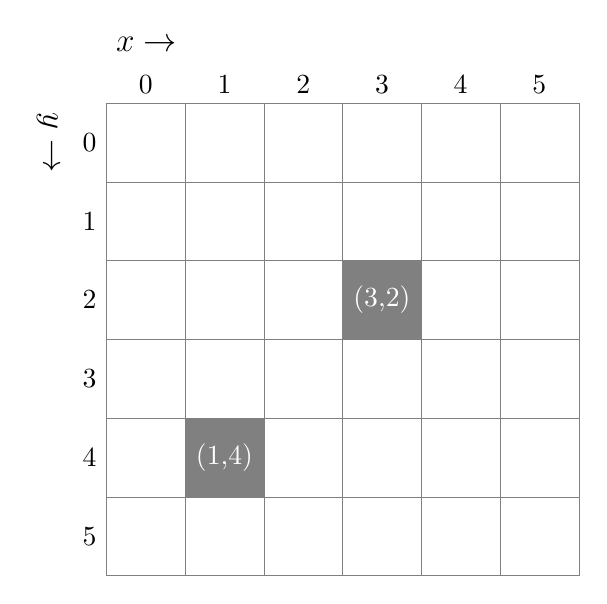
\begin{tikzpicture}

		\node[anchor=west] at (0,6.75) {\large$x\rightarrow$};
		\node[anchor=west,rotate=-90] at (-0.75,6) {\large$y\rightarrow$};

		\foreach \i in {\xMin,...,\xMax} {
			\draw [very thin,gray] (\i,\yMin) -- (\i,\yMax);
		}
		%https://tex.stackexchange.com/questions/36713/computing-in-the-list-of-a-tikz-foreach
		\foreach \i in {\xMin,...,\number\numexpr\xMax-1\relax} {
			\node[anchor=south] at (\i+0.5,\yMax) {$\i$}; 
		}
		\foreach \i in {\yMin,...,\yMax} {
			\draw [very thin,gray] (\xMin,\i) -- (\xMax,\i);
		}
		\foreach \i in {\yMin,...,\number\numexpr\yMax-1\relax} {
			\node[anchor=east] at (\xMin,\yMax - \i-0.5) {$\i$}; 
		}
		\fill [gray] (3,3) rectangle (4,4);
		\node[anchor=center] at (3.5,3.5) {\color{white}(3,2)};
		\fill [gray] (1,1) rectangle (2,2);
		\node[anchor=center] at (1.5,1.5) {\color{white}(1,4)};
	\end{tikzpicture}
	\caption{Pixels in a display occupy space are are referenced to the top left corner with the positive Y axis going down.}
	\label{fig:pixels}
\end{figure}

\section{Using the Display}
The display on the lab board is a 1.3" monochrome display 128 pixels wide and 64 pixels high. Since it is 
monochrome 1 represents white and 0 black for a pixel colors. Two libraries are required to use it:
\begin{enumerate}
	\item \lstinline@Adafruit_GFX.h@ - this is the generic graphics library
	\item \lstinline@Adafruit_SSD1306.h@ - this is specific to our display
\end{enumerate}
An example that shows much of the available functionality can be found (once the libraries are installed)
at Examples $\rightarrow$ Adafruit SSD1306 $\rightarrow$ 128x64 I2C. The following have to be defined to 
use a display:
\begin{enumerate}
	\item Width - how many pixels wide the display is 
	\item Height - how many pixels high the display is 
	\item I2C address - what address the I2C display is accessed at 
	\item Reset pin - not attached to anything on our board so use -1
	\item I2C interface - which I2C interface to communicate over. In our case we only use one, but 
			there are situations where you use more than one I2C interface.
\end{enumerate}
An example of creating a display instance is as follows:\\
\lstinline@Adafruit_SSD1306 display(SCREEN_WIDTH, SCREEN_HEIGHT, &Wire, OLED_RESET);@

Some useful methods that can be called on the display object are:
\begin{enumerate}
	\item clearDisplay - clears everything to black 
	\item display - show whatever has been queued up in the buffer
	\item setTextSize - sets the size of the text (usually 1 or 2)
	\item setTextColor - set what color the text should
	\item print/println - these act the same as they do when using Serial
	\item drawBitmap - draws a bitmap stored using PROGMEM. It requires the following arugments
	\begin{enumerate}
		\item xpos - the x position for the image
		\item ypos - the y position for the image
		\item bitmap variable - the variables with the actual image
		\item width - image width in pixels
		\item height - image height in pixels 
		\item color - color for the nonzero pixels in the image
	\end{enumerate}
	\item more can be \href{https://learn.adafruit.com/adafruit-gfx-graphics-library/graphics-primitives}{found here}.
	\item Functions specific to our display can be \href{https://github.com/adafruit/Adafruit_SSD1306/blob/master/Adafruit_SSD1306.h}{found here}.
\end{enumerate}
The colors for our display are \lstinline@SSD1306_WHITE@ and \lstinline@SSD1306_BLACK@. Note that text normally 
wraps if it is too long for the current line.

\section{Lab Exercise}
\subsection{To Do}
This is an implementation of the display homework. Below is the modified version for lab with some additions 
so read carefully.


Based on the Example \lstinline@ssd1306_128x64_i2c@ and the button programs you have already written, write a 
program for the CEC 326 board that does the following:
\begin{enumerate}
	\item \label{a:display}Displays a custom (written by you) set of text for 2 seconds indicating the start of the program
	\item Moves a custom BMP left with the left button and right with the right button. You can base this 
			off of the \lstinline@testanimate@ function. 
	\item Once you have that working, switch your custom message on boot from \ref{a:display} to display the current
			temperature and humidity from the SHT31. I based my SHT31 code on the Adafruit SHT31 library.
\end{enumerate}
Some thoughts about the process:
\begin{enumerate}
	\item The example code has \lstinline@testanimate@ called inside \lstinline@setup()@. Your function should be called from 
			the loop function. 
	\item Note that the \lstinline@testanimate@ function has an infinite loop inside it. Your function should not 
			have an infinite loop inside it.
	\item Your code should have a proper header at the top
	\item Don't forget to call \lstinline@display.display()@ to actually display something on the screen.
	\item Have your bitmap start at the location \lstinline@(display.width()/2, display.height()/2)@
	\item Check to see if the bitmap has hit the edges of the screen using the \lstinline@display.width()@ and 
			\lstinline@display.height()@ functions.
	\item Approach this one step at a time.
	\item Go back through and double check all your logic.
	\item Ask if you have questions, but be sure to include a copy of the code you have so far.
\end{enumerate}

\subsection{Converting Images for Arduino}
A website for converting images to a format that the Arduino system can use is at 
\href{http://javl.github.io/image2cpp/}{http://javl.github.io/image2cpp/}. I used the following settings:
\begin{enumerate}
	\item Canvas size: 16x16
	\item  Background color: Black
	\item  Invert image color: checked
	\item  Center horizontal and vertical
	\item  Arduino code, single bitmap
	\item  Horizontal - 1 bit per pixel
	\item  Change the name in the code from NaN to something useful.
	\item  reformated it by adding new lines to make it fit nicely
\end{enumerate}

\subsection{Submit}
\begin{enumerate}
	\item Demonstrate your program running to the instructor.
	\item Submit a PDF of your code on Canvas.
\end{enumerate}
